\documentclass[11pt, letterpaper]{article}
\usepackage[utf8]{inputenc} %Paquete de Codificación
\usepackage[spanish]{babel} %Paquete de idioma
\usepackage{enumitem}       %Paquete para listas
\usepackage{graphicx}       %Paquete para imagenas
\usepackage{amsmath}        %Paquete para matematicas
\usepackage{lipsum}         %Paquete para texto aleatorio
\usepackage{hyperref}
\usepackage{listings}
\usepackage{subfig}
\graphicspath{ {img/} }  %Path para carpeta imagenes



\begin{document}

\begin{titlepage}
	\centering
	{\bfseries\LARGE Universidad de Alicante\par}
	\vspace{1cm}
	{\scshape\Large Escuela Politecnica Superior\par}
	\vspace{3cm}
	{\scshape\Huge Entregable 2\par}
	\vspace{3cm}
	\vfill
	{\Large Autor: \par}
	{\Large David Carbonell Pastor \par}
	\vfill
	{\Large 2022\par}
\end{titlepage}

\tableofcontents

\pagebreak

\section{Uso de la plataforma IoT Ubidots}
\subsection{Evidencias del trabajo realizado}
Se ha utilizado la plataforma IoT Ubidots a través de Node-Red como se puede ver en la figura \ref{fig:ubidots_nodered}
de esta manera se simplifica el apartado de la programación ya que de otra manera se ha de realizar mediante codigo python para
lo que pretendemos implementar.
\begin{figure}[h]
	\centering
	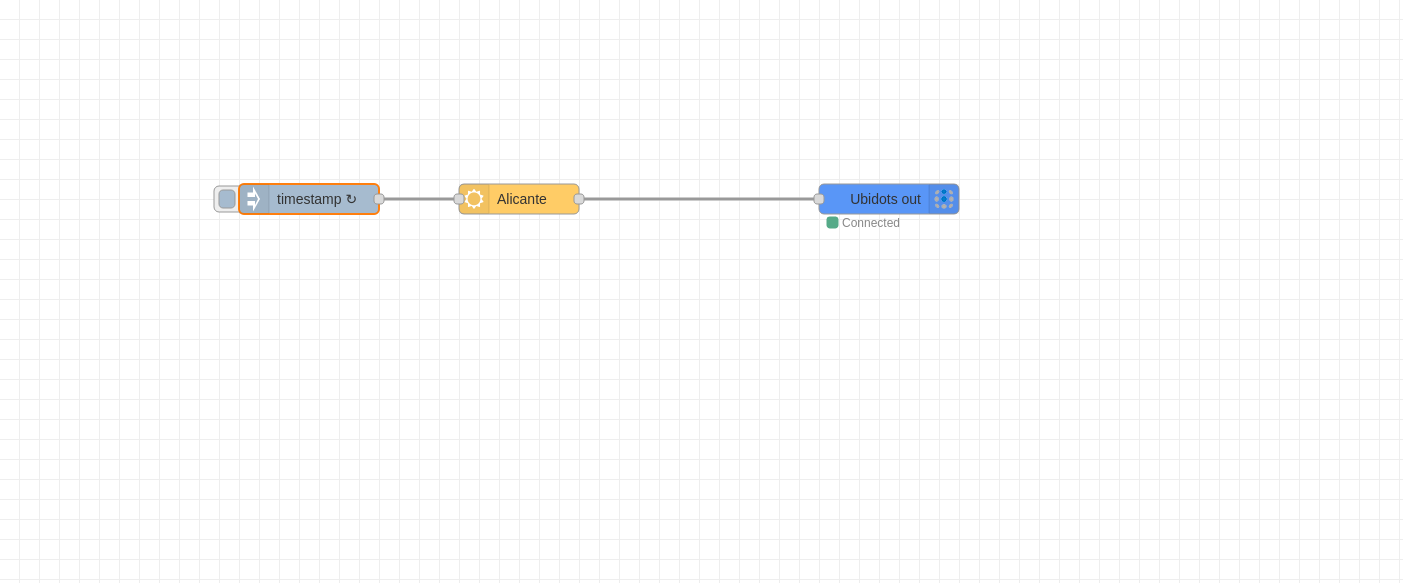
\includegraphics[width=\textwidth]{ubidots_nodered.png}
	\caption{Conexion de ubidots con nodered}
	\label{fig:ubidots_nodered}
\end{figure}

Enviamos la información del nodo de openweather al nodo de ubidots
en la pagina de ubidots en el apartado devices nos aparecen los parametros
que nos proporciona en formato json de una manera mas visual donde podemos ver los
distintos datos que tenemos.\\


Con los datos proporcionados por el nodo de openweather se ha realizado un dashboard simple \ref{fig:dashboard_ejemplo}
el cual presenta una menor complejidad y mayores funcionalidades que los dashboard creados con node-red
en el anterior entregable.

\pagebreak
\begin{figure}[h]
	\centering
	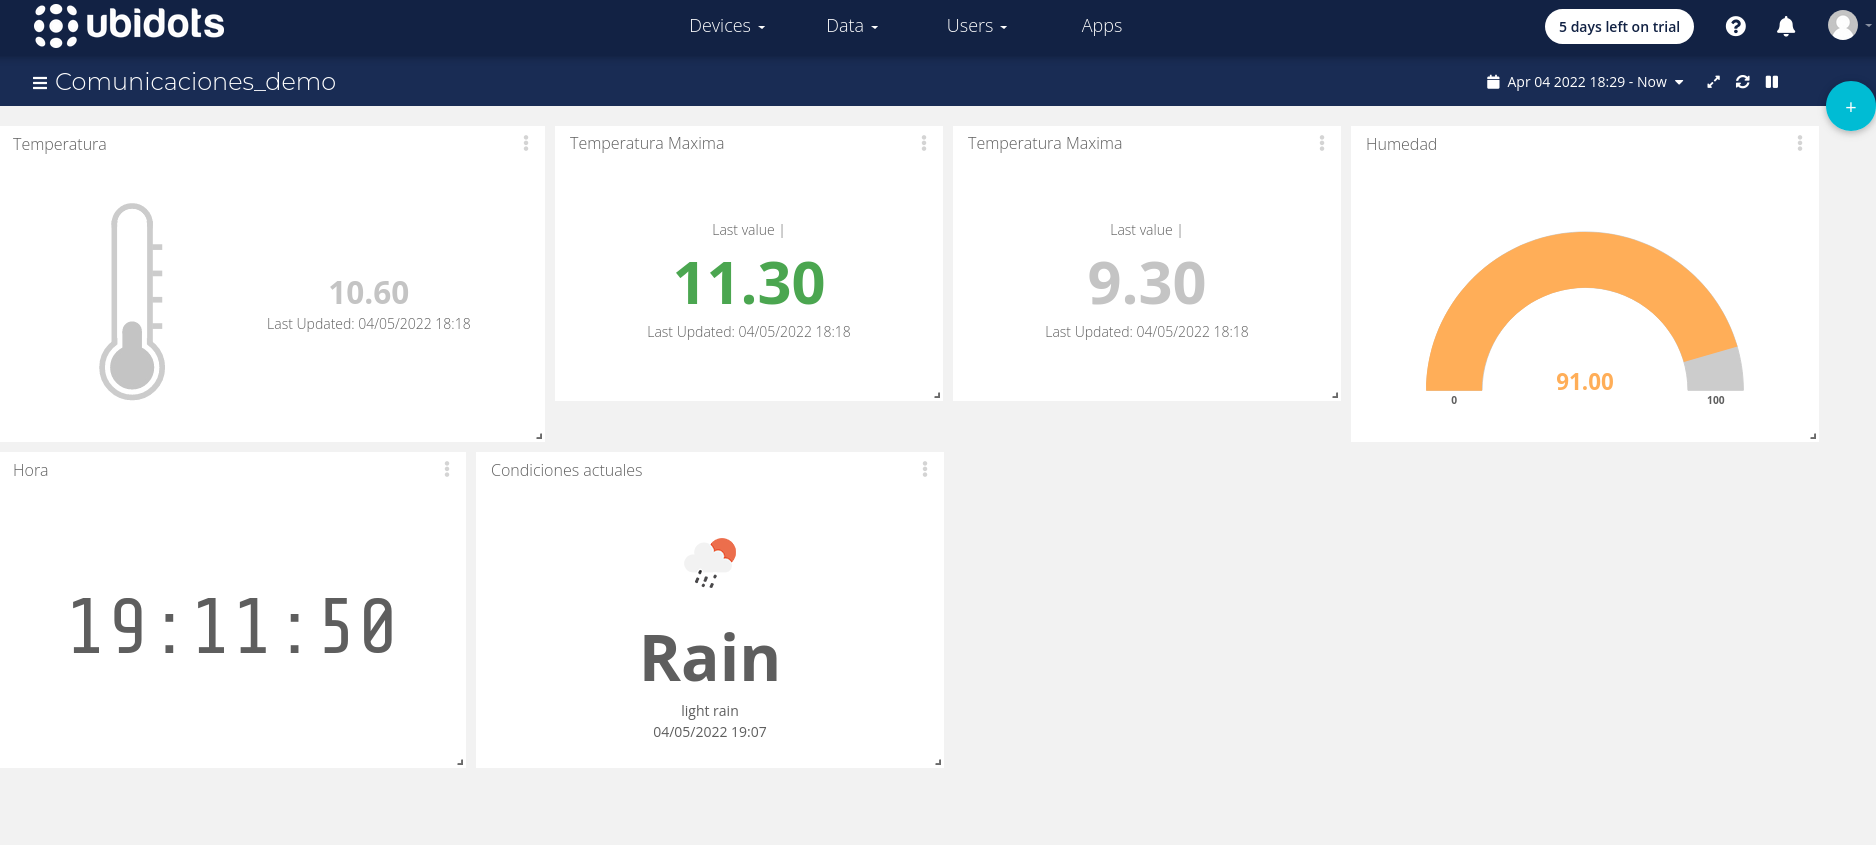
\includegraphics[width=\textwidth]{dashboard_ejemplo.png}
	\caption{Dashboard simple con datos de openweather}
	\label{fig:dashboard_ejemplo}
\end{figure}

Enlace al dashboard creado \url{https://industrial.ubidots.com/app/dashboards/public/dashboard/59mHN0d4o7UrQGhN3BC5KWEvK0hM2c7FXGd-t9ClxBk}

\subsection{Ampliacion de conocimientos}
Se va a realizar una lectura y escritura de datos obtenidos mediante el ESP-32 y la plataforma
ubidots todo el codigo se encuentra adjunto en la practica y en el github para su consulta.
\subsubsection{Enviar valores de del ESP-32 a Ubidots}
Tanto para mandar como para recibir los valores desde el ESP-32 a Ubidots vamos a
utlizar la librería \texttt{UbidotsEsp32Mqtt.h} desde el framework de arduino. El protocolo que utilizamos tanto 
para enviar como recibir los datos es MQTT.


Para mandar los datos a la plataforma Ubidots utlizamos los metodos \texttt{ubidots.add} y \texttt{ubidots.publish}
donde introducimos el nombre del dispositivo y las variables que hemos leido previamente mediante las funciones como puede ser en
nuestro caso \texttt{analogRead()} o \texttt{digitalRead()}.\\

Para saber si la conexion se ha realizado con exito debe aparecer el mensaje de la siguiente figura:

\begin{figure}[h]
	\centering
	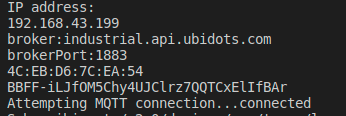
\includegraphics[width=\textwidth]{Mensaje_bienconectado.png}
	\caption{Mensaje debe aparecer en el monitor serie del ESP32}
	\label{fig:mensaje_bien_conectado}
\end{figure}
\pagebreak

Los datos mandados a la Ubidots aparecen de la siguiente forma:
\begin{figure}[h]
	\centering
	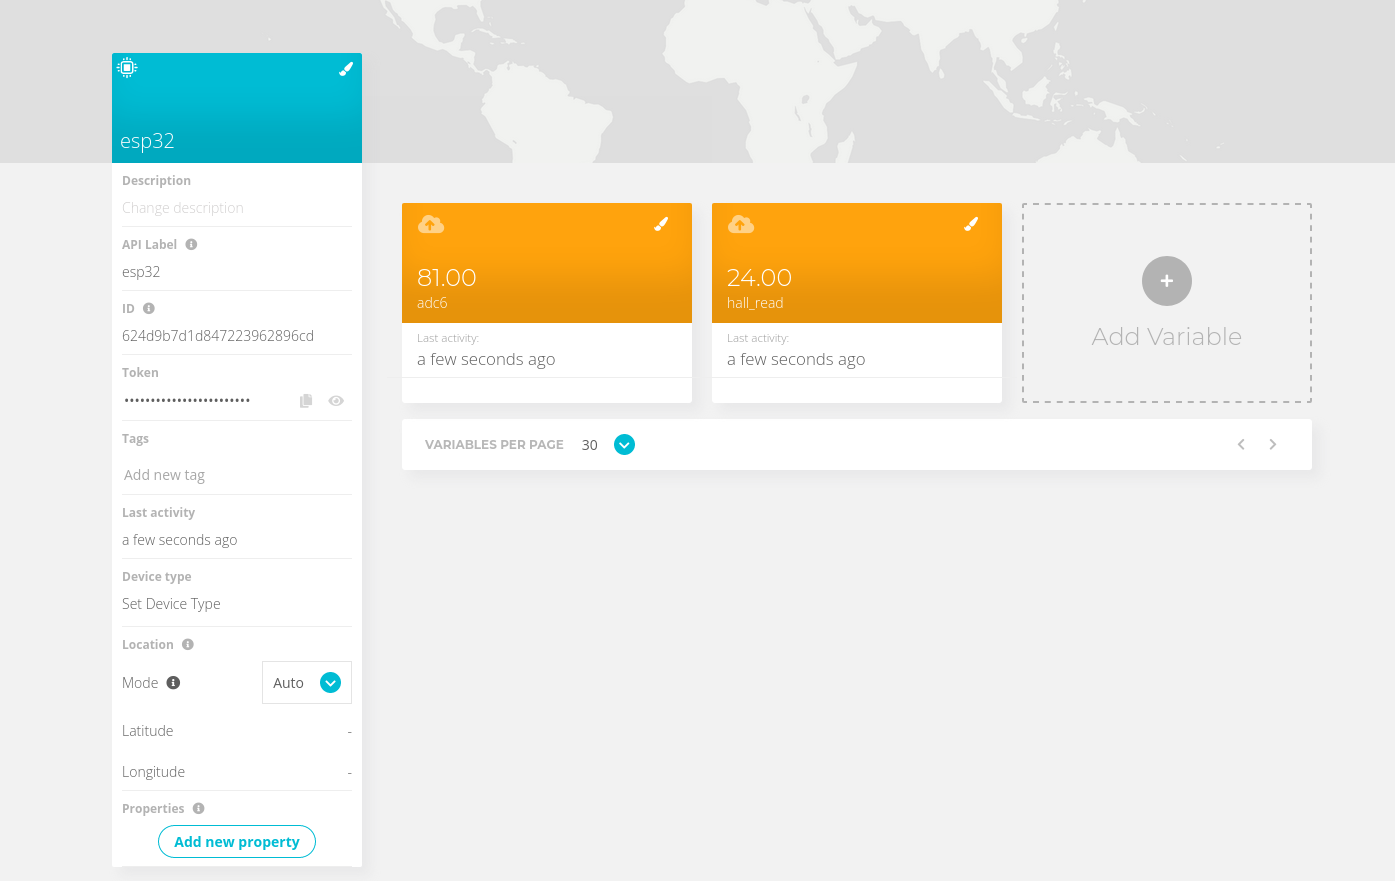
\includegraphics[width=\textwidth]{datos_esp32_ubidots.png}
	\caption{Datos del ADC6 y hall sensor en Ubidots} 
	\label{fig:datos_esp32_ubidots}
\end{figure}
\pagebreak
\begin{figure}[h]
	\centering
	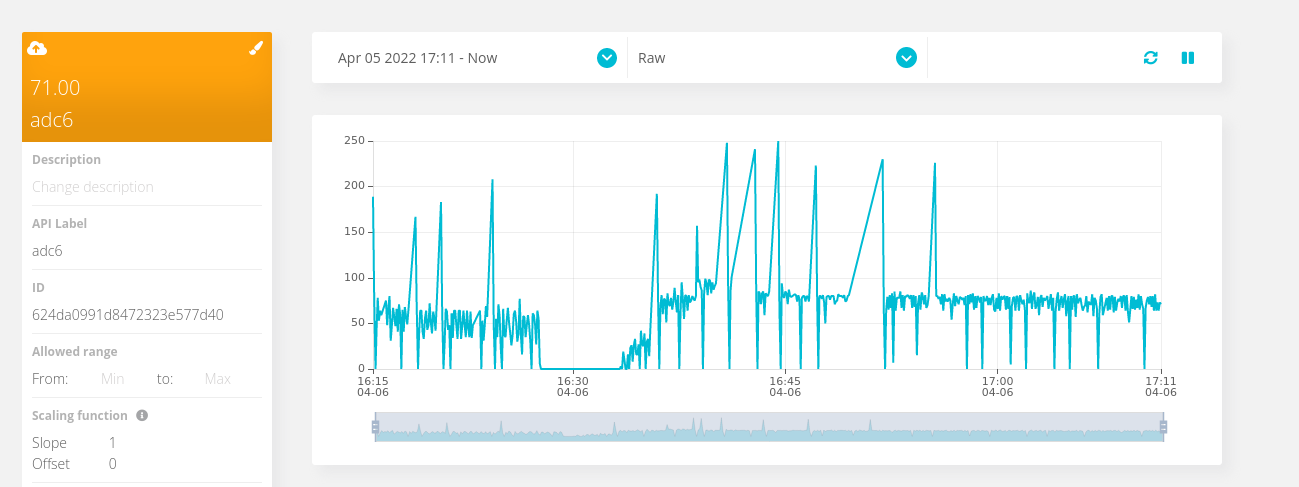
\includegraphics[width=\textwidth]{datos_ADC6.png}
	\caption{Datos proporcionados por el ADC6} 
	\label{fig:datos_esp32_ubidots}
\end{figure}

\subsubsection{Recibir valores de Ubidots a ESP-32}
Para recibir los valores que mandamos a través de node-red a ubidots es un proceso muy similar al de mandar los valores 
en el codigo solamente añadimos la funcion \texttt{ubidots.subscribeLastValue} donde se indica el dispotivo al que nos subscribimos ya la 
variable que queremos leer. Esto no proporciona los valores de la variable por terminal de la siguiente forma:

\begin{figure}[h]
	\centering
	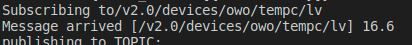
\includegraphics[width=\textwidth]{Temperatura_recibida_ESP32.png}
	\caption{Temperatura leida por el ESP32 a través de Ubidots} 
	\label{fig:temp}
\end{figure}

\section{Uso de relés inteligentes}
\subsection{Configuración de Shelly 1}
Shelly es uno de los dispositivos inteligentes que permiten 
el control por Wifi de la iluminación o los electrodomesticos.
Shelly usa la red wifi para la interconexión de sus dispositivos, esto 
hace que su configuración sea muy fácil y rapida. A continuación \ref*{fig:conexion_Shelly1_red} se muestra un diagrama 
de como realizar su conexionado a la red.

\begin{figure}[h]
	\centering
	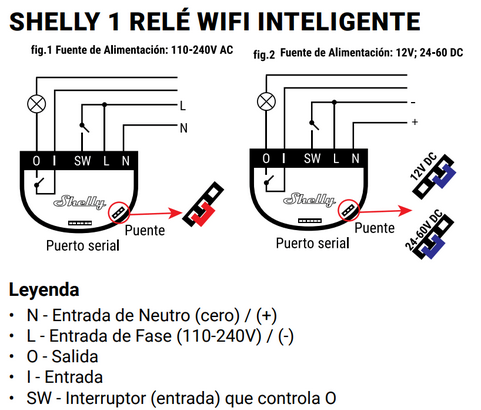
\includegraphics[width=\textwidth]{conexion_Shelly1_red.png}
	\caption{Esquema de conexión de Shelly 1 a la red electrica} 
	\label{fig:conexion_Shelly1_red}
\end{figure}
\pagebreak
Despues de haber realizado la instalación del dispositivo, el mismo crea una red
wifi a la cual debes conectarte para realizar la configuración.
\begin{itemize}
    \item Primero tienes que acceder la web de configuración del 
    dispositivo introduciendo la ip \texttt{192.168.33.1} en el navegador.
    \item Dentro de la web se puede comprobar si es el shelly que queremos configurar apagando y encendiendo el dispositivo.
    \item En el apartado \textit{Internet \& Security} se selecciona \textit{Wifi-Mode-Client} donde se introduce nuestra red wifi que queremos que se conecte el dispositivo.
    \item También se puede realizar la configuración desde la aplicación \textit{Shelly Cloud}.
\end{itemize}

\subsection{Relés con node-red mediante http request}
A través de node-red se pueden controlar los diversos relés que se encuentran conectados a la red, a través
del nodo \texttt{httprequest}.\\


Para ver toda la información \ref{fig:Ver_informacion_rele} que nos proporciona el relé utilizamos el nodo \texttt{httprequest} con la siguiente direccion \texttt{http://192.168.10.110/emeter/0}


\begin{figure}[h]
	\centering
	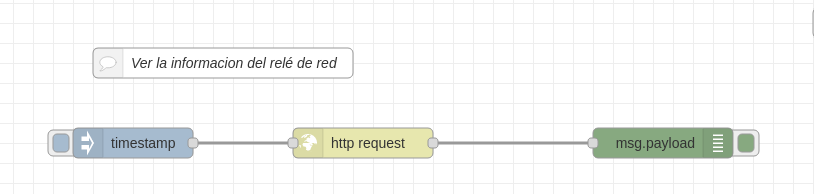
\includegraphics[width=\textwidth]{Ver_informacion_rele.png}
	\caption{Esquema node-red para ver informacón del relé} 
	\label{fig:Ver_informacion_rele}
\end{figure}

Para cambiar el estado \ref{fig:Cambiar_estado_rele} al que se encuentra el relé utilizamos el nodo \texttt{httprequest} con la siguiente direccion \texttt{http://192.168.10.109/relay/0?turn=on}
para cambiar el estado cambiamos el apartado turn a on o off.

\begin{figure}[h]
	\centering
	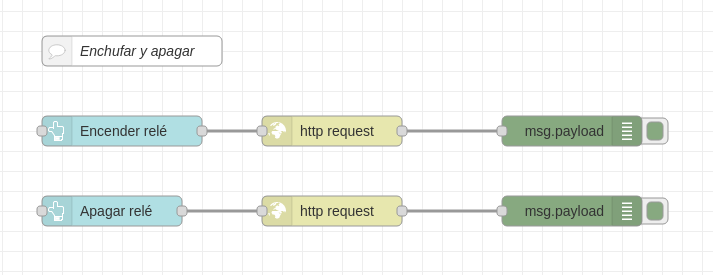
\includegraphics[width=\textwidth]{enchufar_apagar_rele.png}
	\caption{Esquema node-red para cambiar el estado del relé} 
	\label{fig:Cambiar_estado_rele}
\end{figure}

Finalmente se realizó un dashboard \ref{fig:dashboard_rele} en el cual se obtienen los parametros proporcionados por el relé como son la potencia y el voltaje 
los cuales se leen emeter como se ha explicado previamente, para leer solamente los parametros que deseamos se ha utilizado un nodo function 
donde extraemos del \textit{json} esos parametros. También se ha realizado mediante un nodo button que permite encender o apagar el relé de una manera mas sencilla.
\pagebreak
\begin{figure}[h]
	\centering
	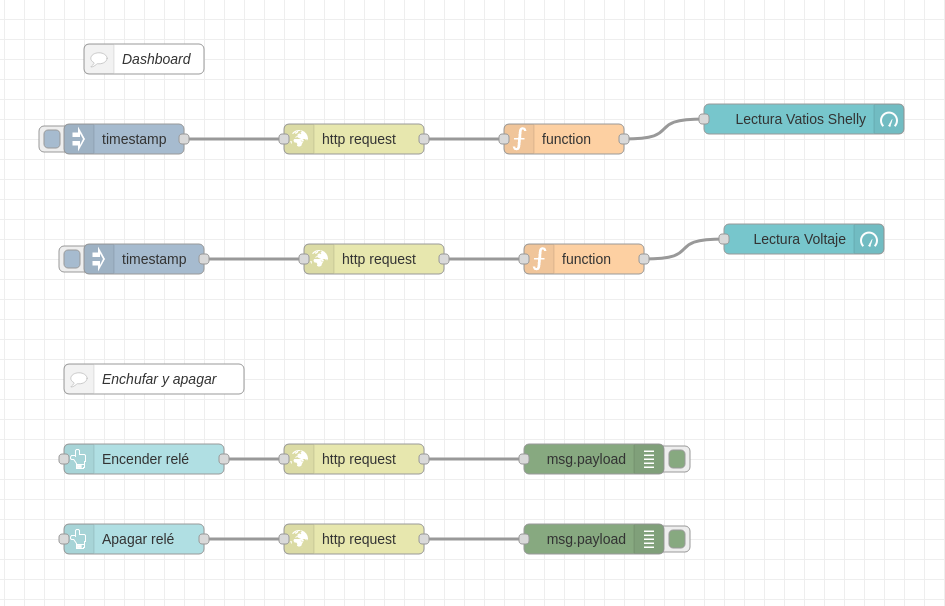
\includegraphics[width=\textwidth]{dashboard_nodos.png}
	\caption{Nodos para realizar el dashboard} 
	\label{fig:Nodos_dashboard}
\end{figure}

\begin{figure}[h]
	\centering
	\includegraphics[width=\textwidth]{dashboard_relé.png}
	\caption{Dashboard de datos y encender el relé} 
	\label{fig:dashboard_rele}
\end{figure}
\pagebreak
De manera extra se probaron también otras funciones de los relés que se encontraban
en el laboratorio. Primero se probó el encender el relé durante 10 segundos \ref{fig:encender_10_sec} mediante la siguiente dirección 
\\\texttt{http://192.168.10.110/relay/0?turn=on\&timer=10} donde en el apartado timer se especifica el tiempo en segundos
que va permanecer encendido el relé.También se probó con el relé que controla la persiana \ref{fig:abrir_persiana} donde se probó a abrirla completamente con
la dirección \texttt{http://192.168.10.110/roller/0?go=open}.Y finalmente a abrir la persiana en un 30 porciento \ref{fig:abrir_30_porciento} mediante la siguiente dirección 
\texttt{http://192.168.10.110/roller/0?go=to\_pos\&roller\_pos=30} 

\begin{figure}[h]
	\centering
	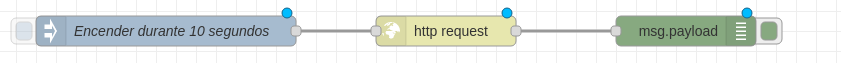
\includegraphics[width=\textwidth]{encender_10_sec.png}
	\caption{Encender relé durante 10 segundos} 
	\label{fig:encender_10_sec}
\end{figure}

\begin{figure}[h]
	\centering
	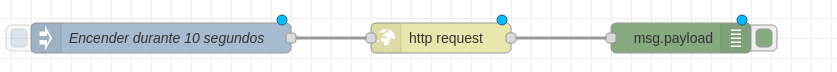
\includegraphics[width=\textwidth]{abrir_persiana.png}
	\caption{Encender el relé de la persiana} 
	\label{fig:abrir_persiana}
\end{figure}

\begin{figure}[h]
	\centering
	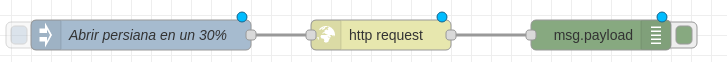
\includegraphics[width=\textwidth]{abrir_persiana_30_porciento.png}
	\caption{Encendemos el relé de la persiana en 30 porciento}
	\label{fig:abrir_30_porciento}
\end{figure}

\subsection{Relés con node-red mediante MQTT}
Como http request presenta limitaciones a la hora de controlar nodos ya que este protocolo al ser una petición http tiende mas 
a caerse o a fallar.Utilizamos el protocolo mqtt que acepta mayor numero de peticiones a la vez y es mas fiable. Para ello al igual que en http request nos
conectamos a la misma red wifi en la que se encuentran los relés pero a diferencia de http request ahora nos conectamos al servidor mqtt que se ha creado en dicha red.
A continuación se muestra un ejemplo de mandar un mensaje y recibirlo mediante mqtt:
\begin{figure}[h]
    \centering
    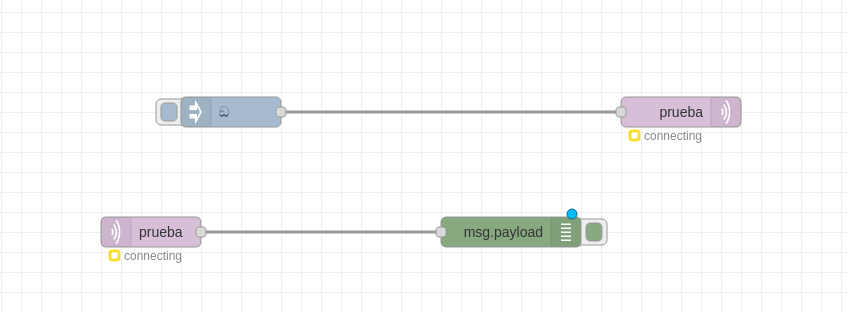
\includegraphics[width=\textwidth]{mqtt_enviar_recibir.png}
    \caption{Enviar y recibir mensajes mediante mqtt} 
    \label{fig:mqtt_enviar_recibir}
\end{figure}

Para obtener la información de los relés mediante \textit{MQTT} se ha utilizado un nodo \texttt{mqtt} que nos permite 
recibir los mensajes de los relés con el topic \texttt{shellies/\#} 

\begin{figure}[h]
    \centering
    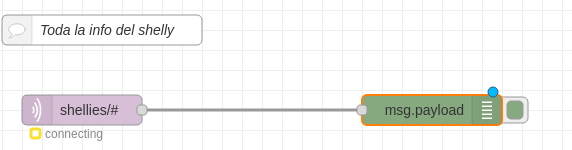
\includegraphics[width=\textwidth]{info_shelly_mqtt.png}
    \caption{Obtener toda la información del relé mediante mqtt} 
    \label{fig:info_shelly_mqtt}
\end{figure}
\pagebreak
Para obtener otro parametros \ref{fig:voltaje_pontencia_mqtt} como pueden ser el voltaje o la potencia, se cambia el topic del nodo mqtt.
Por ejemplo en el caso de la potencia y el voltaje los topics son los siguientes \texttt{shellies/shellyem1/emeter/0/voltage}
\texttt{shellies/shellyem1/emeter/0/power} 

\begin{figure}[h]
    \centering
    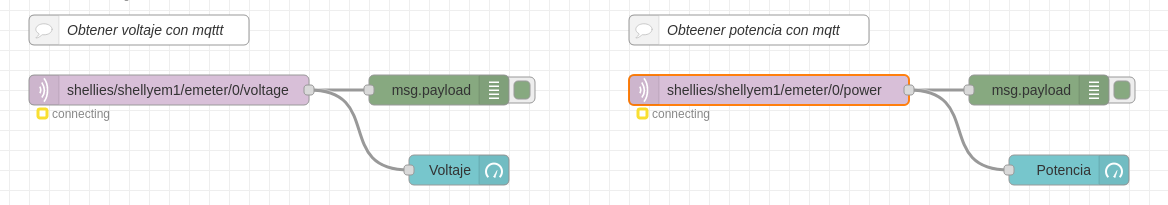
\includegraphics[width=\textwidth]{Voltaje_potencia_mqtt.png}
    \caption{Obtener el voltaje y la potencia del relé mediante mqtt}
    \label{fig:voltaje_pontencia_mqtt}
\end{figure}

También se pueden apagar y encender los relés mediante mqtt al igual que hemos hecho con http request, pero a la hora 
del mundo real mqtt es mucho mas interesante que http request ya que aguanta un mayor numero de llamadas y es mas fiable evitando 
que el relé falle o se caiga la conexión como pudimos ver de manera experimental en el laboratorio con mqtt y toda la gente realizando peticiones
funcionaba de una manera correcta mientras que con http request presentaba alguna caida.\\


A continuación se muestra un ejemplo de como encender y apagar el relé mediante mqtt:

\begin{figure}[h]
    \centering
    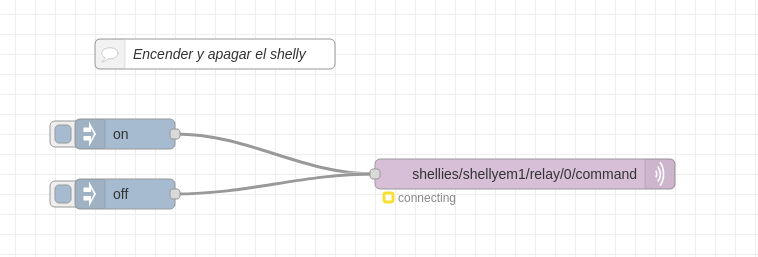
\includegraphics[width=\textwidth]{encender_apagar_mqtt.png}
    \caption{Encender y apagar relé mediante mqtt}
    \label{fig:encender_apagar_mqtt}
\end{figure}
\pagebreak
\section{Ampliación MQTT: Conectar ESP32 a broker MQTT} 
Para esta aplicacion vamos a utlizar un broker gratuito llamado \textit{EMQX} que nos permite conectar nuestra aplicación a un broker mqtt.
La propia web nos ofrece un interfaz \ref{fig:intefaz_web} en la cual podemos ver los diversos mensajes que nos llega o enviamos a través de MQTT.
Se ha realizado una prueba mediante node-red para probar las funcionalidades que presenta, en este caso se ha probado mandar mensajes como aparecen
a continuación:

\begin{figure}[h]
    \centering
    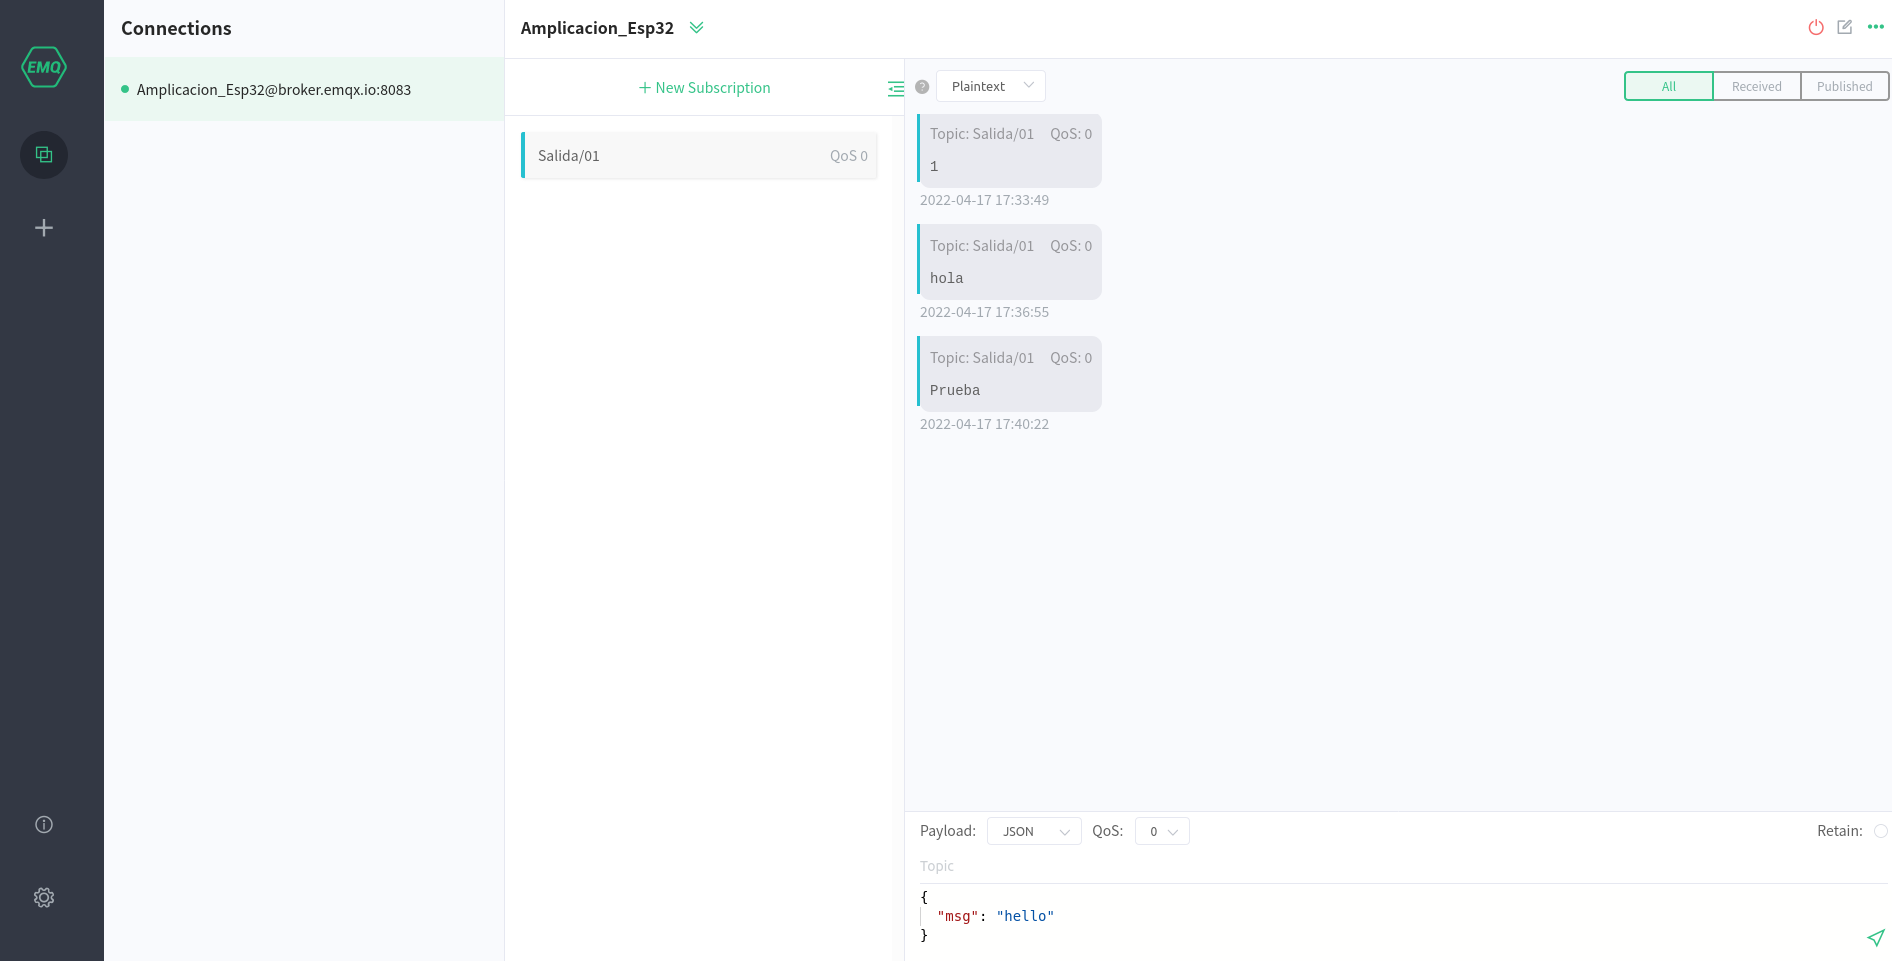
\includegraphics[width=\textwidth]{Captura_mqtt_prueba.png}
    \caption{Prueba de la interfaz que nos ofrece el broker MQTT}
    \label{fig:intefaz_web}
\end{figure}

La aplicacion que vamos a hacer es leer el valor de adc6 y mandarlo al broker mqtt, para ello hacemos uso 
de las librerías \texttt{Wifi.h} y \texttt{PubSubClient.h} que nos permiten conectarnos con el ESP-32 a través de wifi 
al broker.

Finalmente obtenemos el siguiente resultado por puerto serie \ref{fig:puerto_serie} y este resultado en la web del broker mqtt \ref{fig:resultado_web}
no coincide el valor del adc al ser un broker publico le llegan los valores con cierto retraso y el que aparece es el de una prueba anterior.

\begin{figure}[h]
    \centering
    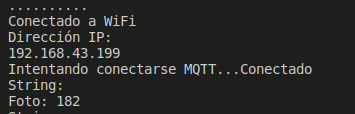
\includegraphics[width=\textwidth]{puerto_serie.png}
    \caption{Informacion que nos muestra el esp32 en el puerto serie}
    \label{fig:puerto_serie}
\end{figure}


\begin{figure}[h]
    \centering
    
\includegraphics[width=\textwidth]{Resultado_broker.png}
    \caption{Valor del adc en el broker mqtt}
    \label{fig:resultado_web}
\end{figure}


\section{Conclusiones}
En el desarrollo de esta practica se ha conseguido aprender a utliziar plataformas IoT como en nuestro caso
ubidots.Además de profundizar en el uso de relés inteligentes y sus diversas funcionalidad y protocolos de comunicacion. Finalmente se ha aprendido
a utilizar el protocolo MQTT para comunicarnos con otros dispotivos y sensores de la red.


\pagebreak
\section{Bibliografia}

\url{https://help.ubidots.com/en/articles/748067-connect-an-esp32-devkitc-to-ubidots-over-mqtt}\\
\url{https://industrial.ubidots.com}\\
\url{https://www.hackster.io/shahizat005/building-an-esp32-based-iot-weather-station-with-ubidots-05adcc}\\
\url{https://www.emqx.com/en/mqtt/public-mqtt5-broker}\\

\end{document}